% !TeX root = booklet-01.tex
\section{قواعد هندسی \lr{Layout}}
\label{sec:layout-rules}
\subsection{عرض، فاصله و پوشش را جدا کنیم}
\lr{Minimum Width} حداقل عرض یک ناحیه است؛ عرض خیلی کم می‌تواند ساخت
رسانای پیوسته را نامطمئن کند.
\lr{Minimum Spacing} فاصله لبه‌به‌لبه دو شکل است؛ فاصله کم خطر اتصال
ناخواسته یا نقض محدودیت‌های ساخت را ایجاد می‌کند.
\lr{Enclosure} مقدار پوشش لایه پیرامون شکل لایه دیگر، مثلاً فلز پیرامون
\lr{Contact} است؛ \lr{Overlap/Extension} امتداد لازم یک شکل از لبه شکل دیگر را بیان می‌کند.
این‌ها نقش‌های متفاوتی دارند و با فاصله مرکزبه‌مرکز یکسان نیستند
\cite[بخش \secnum{۱.۵.۳}]{weste}.

در شکل \ref{fig:layout-spacing}، دو خط با عرض \(w\) و فاصله آزاد \(s\)
داریم. فاصله مرکز دو خط برابر \(p=w+s\) است و \lr{Pitch} نامیده می‌شود.
اگر عرض‌ها متفاوت باشند، فاصله مرکزها \(w_1/2+s+w_2/2\) خواهد بود.

\begin{figure}[ht]
\centering
\begin{latin}
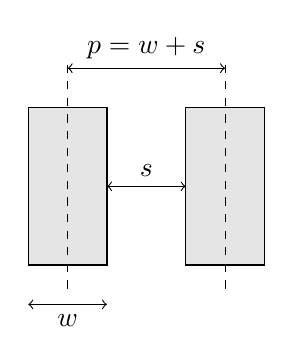
\begin{tikzpicture}[x=1cm,y=1cm]
\draw[fill=gray!20] (0,0) rectangle (1,2);
\draw[fill=gray!20] (2,0) rectangle (3,2);
\draw[dashed] (0.5,-0.3)--(0.5,2.6) (2.5,-0.3)--(2.5,2.6);
\draw[<->] (0,-0.5)--node[below] {$w$}(1,-0.5);
\draw[<->] (1,1)--node[above] {$s$}(2,1);
\draw[<->] (0.5,2.5)--node[above] {$p=w+s$}(2.5,2.5);
\end{tikzpicture}
\end{latin}
\caption{نمای آموزشی عرض، فاصله آزاد و \lr{Pitch}؛ خط‌چین‌ها محور میانی دو خط‌اند.}
\label{fig:layout-spacing}
\end{figure}

\subsection{معنای پارامتر \texorpdfstring{\(\lambda\)}{lambda}}
در قواعد مقیاس‌پذیر آموزشی، طول‌ها به صورت ضریبی از \(\lambda\) نوشته می‌شوند.
در قرارداد این فصل، حداقل طول ترانزیستور رسم‌شده معمولاً \(L_{\min}=2\lambda\)
است. بنابراین انتخاب \(\lambda\) مقیاس فیزیکی نقشه را تعیین می‌کند
\cite[صفحات چاپی ۲۴ و ۲۵]{weste}.
\(\lambda\) در اینجا واحد طول قراردادی است و نباید آن را با ضریب
\lr{Channel Length Modulation} که ممکن است همین حرف را داشته باشد اشتباه گرفت.

\textbf{مثال آموزشی تبدیل مقیاس.} اگر برای مدلی
\(L_{\min}=\qty{0.6}{\micro\metre}\) انتخاب شود، داریم:
\begin{equation}\label{eq:layout-lambda}
\lambda=\frac{L_{\min}}{2}=\qty{0.3}{\micro\metre},\qquad
4\lambda=\qty{1.2}{\micro\metre}.
\end{equation}
ابتدا مقدار فیزیکی یک \(\lambda\) را یافتیم؛ سپس در ضریب هندسی ضرب کردیم.
برای نمونه تاریخی حداقل طول \(\qty{180}{\nano\metre}\)، قرارداد ساده
\(\lambda=\qty{90}{\nano\metre}\) می‌دهد. کتاب در پانوشت توضیح می‌دهد
که حتی برای فرایندهای هم‌نام نیز قرارداد دقیق می‌تواند متفاوت باشد.

این مدل برای یادگیری هندسه و مقیاس مفید است؛ همه قواعد واقعی با یک ضریب
یکسان کوچک نمی‌شوند. نام یک \lr{Technology Node} نیز به‌تنهایی
جدول قابل‌اعمال \lr{Design Rules} را مشخص نمی‌کند.
برای ساخت واقعی باید قواعد و لایه‌های همان \lr{Process Design Kit (PDK)} به کار روند؛
در این جزوه از \lr{PDK} خاصی استفاده نشده است.

\subsection{قواعد ساده کتاب و دامنه کاربردشان}
جدول \ref{tab:layout-rules} خلاصه قواعد ساده و محافظه‌کارانه کتاب برای
مدل \lr{n-well} با دو لایه فلزی است
\cite[صفحات چاپی ۲۵ و ۲۶، شکل \secnum{۱.۳۹}]{weste}.
این جدول تمام قواعد یک فرایند نیست و به معنای تایید ساخت یک \lr{Layout} کامل نیست.

\begin{table}[ht]
\centering
\caption{قواعد آموزشی مبتنی بر \(\lambda\)، برگرفته از کتاب؛ همه اعداد ضرایب \(\lambda\) هستند.}
\label{tab:layout-rules}
\begin{tabularx}{\textwidth}{Xc}
\toprule
ویژگی & مقدار\\
\midrule
حداقل عرض و فاصله آزاد فلز و \lr{Diffusion} & \(4\lambda\)\\
اندازه \lr{Contact} & \(2\lambda\times2\lambda\)\\
پوشش لازم اطراف \lr{Contact} در لایه‌های بالا و پایین & \(1\lambda\)\\
عرض \lr{Poly} & \(2\lambda\)\\
امتداد \lr{Poly} از مرز \lr{Diffusion} در محل ترانزیستور & \(2\lambda\)\\
فاصله \lr{Poly} از \lr{Diffusion} در محل بدون ترانزیستور & \(1\lambda\)\\
فاصله آزاد \lr{Poly}ها و فاصله تماس از \lr{Poly} یا تماس دیگر & \(3\lambda\)\\
پوشش چاه پیرامون \lr{pMOS} و فاصله چاه از \lr{nMOS} & \(6\lambda\)\\
\bottomrule
\end{tabularx}
\end{table}

برای ترانزیستور، \lr{Poly} باید ناحیه فعال را کامل قطع کند و از دو لبه آن
به‌اندازه لازم بیرون بزند؛ این امتداد جلوی باقی‌ماندن مسیر ناخواسته دور \lr{Gate}
را می‌گیرد. اگر ترانزیستور نمی‌خواهیم، باید فاصله آزاد را حفظ کنیم؛
تقاطع تصادفی \lr{Poly} و \lr{Active} می‌تواند قطعه ناخواسته بسازد.

\lr{Contact} باید از هر طرف با لایه‌های مجاز پوشانده شود؛ صرف قرار گرفتن
مرکز آن داخل فلز کافی نیست. از جدول می‌توان حداقل عرض ناحیه تماس‌پذیر را استخراج کرد:
\begin{equation}\label{eq:layout-contact}
w_{\mathrm{landing}}=1\lambda+2\lambda+1\lambda=4\lambda.
\end{equation}
شکل \ref{fig:layout-contact} این محاسبه را برای یک بعد نشان می‌دهد؛
در بعد دیگر نیز همین پوشش لازم است.

\begin{figure}[ht]
\centering
\begin{latin}
% Dimension values remain Persian even in the Latin diagram environment.
\PersianMathDigits
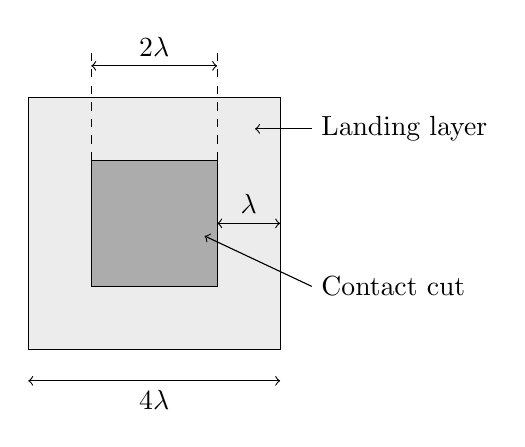
\begin{tikzpicture}[x=0.8cm,y=0.8cm]
\draw[fill=gray!15] (0,0) rectangle (4,4);
\draw[fill=gray!65] (1,1) rectangle (3,3);
\draw[<->] (0,-0.5)--node[below] {$4\lambda$}(4,-0.5);
\draw[<->] (1,4.5)--node[above] {$2\lambda$}(3,4.5);
\draw[dashed] (1,3)--(1,4.7) (3,3)--(3,4.7);
\draw[<->] (3,2)--node[above] {$\lambda$}(4,2);
\node[right] at (4.5,3.5) {Landing layer};
\draw[->] (4.5,3.5)--(3.6,3.5);
\node[right] at (4.5,1) {Contact cut};\draw[->] (4.5,1)--(2.8,1.8);
\end{tikzpicture}
\end{latin}
\caption{مثال اندازه‌دار برای رابطه \eqref{eq:layout-contact}.
مربع داخلی، محل برش تماس و مربع بیرونی، مرز حداقل لایه پوشاننده است؛
لایه دیگر اتصال نیز باید پوشش و قواعد مستقل خود را داشته باشد.}
\label{fig:layout-contact}
\end{figure}

اگر دو تماس \(2\lambda\) در امتداد عرض کنار هم و با فاصله آزاد
\(3\lambda\) قرار گیرند و در دو طرف \(1\lambda\) پوشش داشته باشند،
طول ناحیه لازم \((1+2+3+2+1)\lambda=9\lambda\) می‌شود.
این استدلال، مقدار ذکرشده در پانوشت کتاب برای تماس دوگانه را روشن می‌کند؛
دو تماس می‌توانند افزونگی اتصال را بهتر کنند، ولی صحت همه قواعد فرایند را تضمین نمی‌کنند.

\subsection{طول و عرض ترانزیستور را از کدام جهت بخوانیم؟}
طول کانال \(L\)، فاصله مسیر جریان زیر \lr{Gate} میان دو سوی
\lr{Source/Drain} است. عرض کانال \(W\)، اندازه عمود بر این مسیر در ناحیه
\lr{Gate} روی \lr{Active} است.
پس اگر \lr{Active} افقی و \lr{Poly} عمودی باشد، عرض افقی نوار \lr{Poly}
طول کانال و ارتفاع نوار \lr{Active} عرض کانال را تعیین می‌کند؛
شکل \ref{fig:layout-wl} برای همین جهت رسم شده است.

\begin{figure}[ht]
\centering
\begin{latin}
\PersianMathDigits
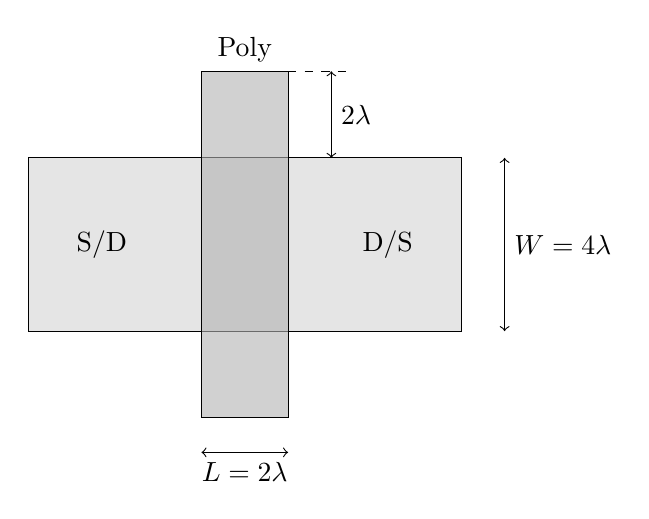
\begin{tikzpicture}[x=0.55cm,y=0.55cm]
\draw[fill=gray!20] (0,0) rectangle (10,4);
\draw[fill=gray!60,fill opacity=0.6] (4,-2) rectangle (6,6);
\node at (1.7,2) {S/D};\node at (8.3,2) {D/S};
\node[above] at (5,6) {Poly};
\draw[<->] (4,-2.8)--node[below] {$L=2\lambda$}(6,-2.8);
\draw[<->] (11,0)--node[right] {$W=4\lambda$}(11,4);
\draw[<->] (7,4)--node[right] {$2\lambda$}(7,6);
\draw[dashed] (6,4)--(7.5,4) (6,6)--(7.5,6);
\end{tikzpicture}
\end{latin}
\caption{طرح هندسی آموزشی یک کانال با \(W=4\lambda\) و \(L=2\lambda\).
امتداد \lr{Poly} از ناحیه فعال نیز نشان داده شده است؛ تماس‌های \lr{Source/Drain}
در این شکل حذف شده‌اند و شکل، \lr{Layout} کامل تماس‌دار نیست.}
\label{fig:layout-wl}
\end{figure}

نماد \(W/L=4/2\) در شکل‌های آموزشی کتاب یعنی \(W=4\lambda\) و
\(L=2\lambda\)، نه فقط نسبت عددی ۲ بدون مشخص بودن ابعاد.
ترانزیستورهای \(4/2\) و \(8/4\) نسبت یکسان دارند، ولی هندسه و ظرفیت‌هایشان
یکسان نیست. در مدل نمونه رابطه \eqref{eq:layout-lambda}،
\(4/2\) به \(\qty{1.2}{\micro\metre}/\qty{0.6}{\micro\metre}\) تبدیل می‌شود.

کتاب یک \lr{Unit Inverter} با \lr{nMOS} به ابعاد \(4/2\) و \lr{pMOS}
به ابعاد \(8/2\) نشان می‌دهد. حفره‌ها در مدل مورد بحث \lr{Mobility}
کمتری دارند؛ افزایش عرض \lr{pMOS} می‌تواند این تفاوت جریان را تا حدی جبران کند.
ضریب دو در این شکل یک انتخاب آموزشی است؛ قانون ثابت همه فناوری‌ها یا شرط لازم
برای درست بودن جدول منطقی \lr{Inverter} نیست
\cite[شکل \secnum{۱.۴۰}]{weste}.

\subsection{مثال‌های عددی و کنترل مستقل قواعد}
\begin{enumerate}
\item \textbf{دو خط فلزی با عرض \(4\lambda\) و فاصله محور \(7\lambda\):}
فاصله آزاد \(7\lambda-4\lambda=3\lambda\) است؛
قاعده \(4\lambda\) فاصله آزاد نقض شده است، حتی اگر عرض هر دو درست باشد.
\item \textbf{تماس \(2\lambda\) در ناحیه متقارن \(3\lambda\):}
پوشش هر طرف \((3-2)\lambda/2=0.5\lambda\) است؛
از \(1\lambda\) لازم کمتر است و کافی نیست.
\item \textbf{دو خط با عرض و فاصله \(4\lambda\):}
\lr{Pitch} برابر \(8\lambda\) است؛ با \(\lambda=\qty{0.3}{\micro\metre}\)
به \(\qty{2.4}{\micro\metre}\) تبدیل می‌شود.
\end{enumerate}
این کنترل‌ها فقط همان شرط محلی را می‌آزمایند؛ تایید عرض یک خط به معنی
تایید فاصله چاه، نوع تماس، اتصال مدار یا کل \lr{DRC} نیست.
